\chapter{Conspiracy}

Danglars followed Edmond and Mercédès with his eyes until the two
lovers disappeared behind one of the angles of Fort Saint Nicolas;
then, turning round, he perceived Fernand, who had fallen, pale and
trembling, into his chair, while Caderousse stammered out the words of
a drinking-song.

“Well, my dear sir,” said Danglars to Fernand, “here is a marriage
which does not appear to make everybody happy.”

“It drives me to despair,” said Fernand.

“Do you, then, love Mercédès?”

“I adore her!”

“For long?”

“As long as I have known her—always.”

“And you sit there, tearing your hair, instead of seeking to remedy
your condition; I did not think that was the way of your people.”

“What would you have me do?” said Fernand.

“How do I know? Is it my affair? I am not in love with Mademoiselle
Mercédès; but for you—in the words of the gospel, seek, and you shall
find.”

“I have found already.”

“What?”

“I would stab the man, but the woman told me that if any misfortune
happened to her betrothed, she would kill herself.”

“Pooh! Women say those things, but never do them.”

“You do not know Mercédès; what she threatens she will do.”

“Idiot!” muttered Danglars; “whether she kill herself or not, what
matter, provided Dantès is not captain?”

“Before Mercédès should die,” replied Fernand, with the accents of
unshaken resolution, “I would die myself!”

“That’s what I call love!” said Caderousse with a voice more tipsy than
ever. “That’s love, or I don’t know what love is.”

“Come,” said Danglars, “you appear to me a good sort of fellow, and
hang me, I should like to help you, but——”

“Yes,” said Caderousse, “but how?”

“My dear fellow,” replied Danglars, “you are three parts drunk; finish
the bottle, and you will be completely so. Drink then, and do not
meddle with what we are discussing, for that requires all one’s wit and
cool judgment.”

“I—drunk!” said Caderousse; “well that’s a good one! I could drink four
more such bottles; they are no bigger than cologne flasks. Père
Pamphile, more wine!”

And Caderousse rattled his glass upon the table.

“You were saying, sir——” said Fernand, awaiting with great anxiety the
end of this interrupted remark.

“What was I saying? I forget. This drunken Caderousse has made me lose
the thread of my sentence.”

“Drunk, if you like; so much the worse for those who fear wine, for it
is because they have bad thoughts which they are afraid the liquor will
extract from their hearts;” and Caderousse began to sing the two last
lines of a song very popular at the time:

‘Tous les méchants sont buveurs d’eau;

C’est bien prouvé par le déluge.’1


“You said, sir, you would like to help me, but——”

“Yes; but I added, to help you it would be sufficient that Dantès did
not marry her you love; and the marriage may easily be thwarted,
methinks, and yet Dantès need not die.”

“Death alone can separate them,” remarked Fernand.

“You talk like a noodle, my friend,” said Caderousse; “and here is
Danglars, who is a wide-awake, clever, deep fellow, who will prove to
you that you are wrong. Prove it, Danglars. I have answered for you.
Say there is no need why Dantès should die; it would, indeed, be a pity
he should. Dantès is a good fellow; I like Dantès. Dantès, your
health.”

Fernand rose impatiently. “Let him run on,” said Danglars, restraining
the young man; “drunk as he is, he is not much out in what he says.
Absence severs as well as death, and if the walls of a prison were
between Edmond and Mercédès they would be as effectually separated as
if he lay under a tombstone.”

\begin{figure}[h]
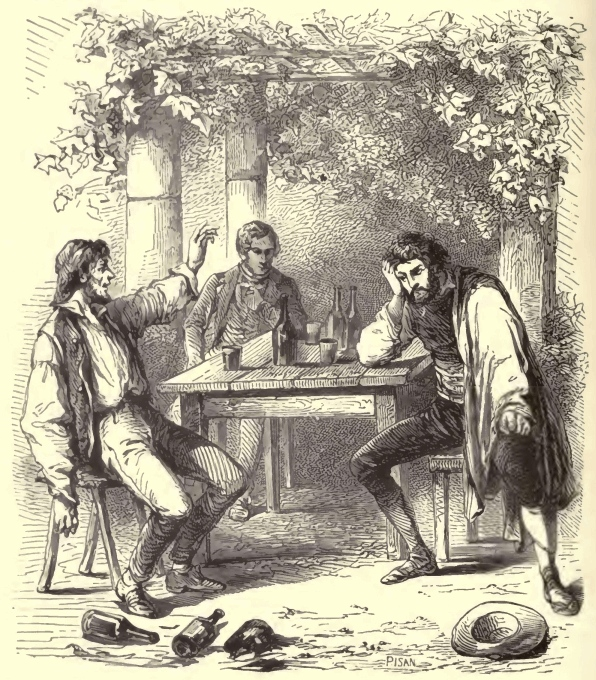
\includegraphics[width=\textwidth]{0056m.jpg}
\end{figure}

“Yes; but one gets out of prison,” said Caderousse, who, with what
sense was left him, listened eagerly to the conversation, “and when one
gets out and one’s name is Edmond Dantès, one seeks revenge——”

“What matters that?” muttered Fernand.

“And why, I should like to know,” persisted Caderousse, “should they
put Dantès in prison? he has neither robbed, nor killed, nor murdered.”

“Hold your tongue!” said Danglars.

“I won’t hold my tongue!” replied Caderousse; “I say I want to know why
they should put Dantès in prison; I like Dantès; Dantès, your health!”
and he swallowed another glass of wine.

\begin{figure}[h]
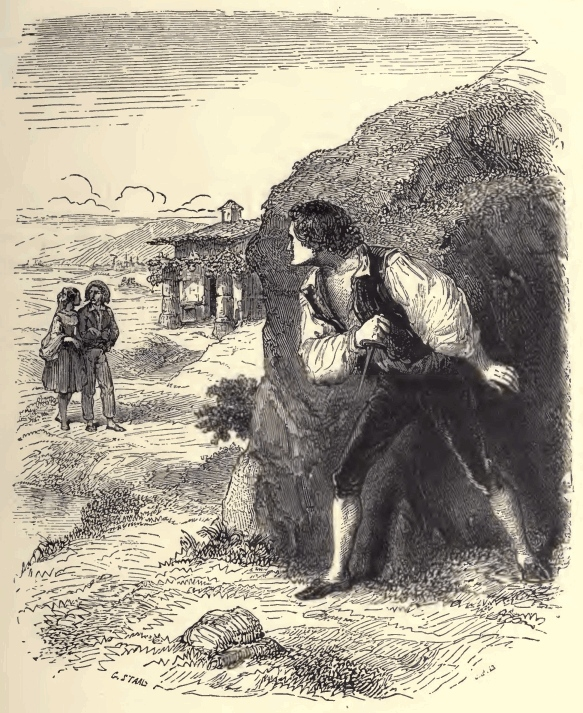
\includegraphics[width=\textwidth]{0057m.jpg}
\end{figure}

Danglars saw in the muddled look of the tailor the progress of his
intoxication, and turning towards Fernand, said, “Well, you understand
there is no need to kill him.”

“Certainly not, if, as you said just now, you have the means of having
Dantès arrested. Have you that means?”

“It is to be found for the searching. But why should I meddle in the
matter? it is no affair of mine.”

“I know not why you meddle,” said Fernand, seizing his arm; “but this I
know, you have some motive of personal hatred against Dantès, for he
who himself hates is never mistaken in the sentiments of others.”

“I! motives of hatred against Dantès? None, on my word! I saw you were
unhappy, and your unhappiness interested me; that’s all; but since you
believe I act for my own account, adieu, my dear friend, get out of the
affair as best you may;” and Danglars rose as if he meant to depart.

“No, no,” said Fernand, restraining him, “stay! It is of very little
consequence to me at the end of the matter whether you have any angry
feeling or not against Dantès. I hate him! I confess it openly. Do you
find the means, I will execute it, provided it is not to kill the man,
for Mercédès has declared she will kill herself if Dantès is killed.”

Caderousse, who had let his head drop on the table, now raised it, and
looking at Fernand with his dull and fishy eyes, he said, “Kill Dantès!
who talks of killing Dantès? I won’t have him killed—I won’t! He’s my
friend, and this morning offered to share his money with me, as I
shared mine with him. I won’t have Dantès killed—I won’t!”

“And who has said a word about killing him, muddlehead?” replied
Danglars. “We were merely joking; drink to his health,” he added,
filling Caderousse’s glass, “and do not interfere with us.”

“Yes, yes, Dantès’ good health!” said Caderousse, emptying his glass,
“here’s to his health! his health—hurrah!”

“But the means—the means?” said Fernand.

“Have you not hit upon any?” asked Danglars.

“No!—you undertook to do so.”

“True,” replied Danglars; “the French have the superiority over the
Spaniards, that the Spaniards ruminate, while the French invent.”

“Do you invent, then,” said Fernand impatiently.

“Waiter,” said Danglars, “pen, ink, and paper.”

“Pen, ink, and paper,” muttered Fernand.

“Yes; I am a supercargo; pen, ink, and paper are my tools, and without
my tools I am fit for nothing.”

“Pen, ink, and paper, then,” called Fernand loudly.

“There’s what you want on that table,” said the waiter.

“Bring them here.” The waiter did as he was desired.

\begin{figure}[h]
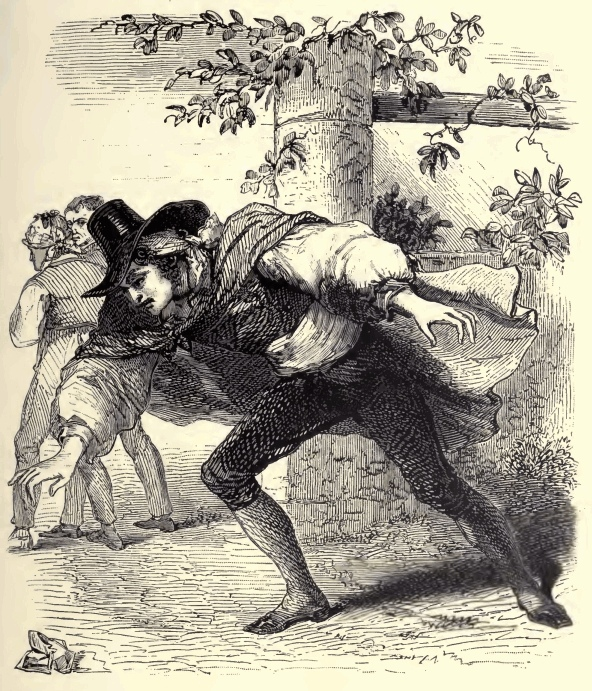
\includegraphics[width=\textwidth]{0059m.jpg}
\end{figure}

“When one thinks,” said Caderousse, letting his hand drop on the paper,
“there is here wherewithal to kill a man more sure than if we waited at
the corner of a wood to assassinate him! I have always had more dread
of a pen, a bottle of ink, and a sheet of paper, than of a sword or
pistol.”

“The fellow is not so drunk as he appears to be,” said Danglars. “Give
him some more wine, Fernand.” Fernand filled Caderousse’s glass, who,
like the confirmed toper he was, lifted his hand from the paper and
seized the glass.

The Catalan watched him until Caderousse, almost overcome by this fresh
assault on his senses, rested, or rather dropped, his glass upon the
table.

“Well!” resumed the Catalan, as he saw the final glimmer of
Caderousse’s reason vanishing before the last glass of wine.

“Well, then, I should say, for instance,” resumed Danglars, “that if
after a voyage such as Dantès has just made, in which he touched at the
Island of Elba, someone were to denounce him to the king’s procureur as
a Bonapartist agent——”

“I will denounce him!” exclaimed the young man hastily.

“Yes, but they will make you then sign your declaration, and confront
you with him you have denounced; I will supply you with the means of
supporting your accusation, for I know the fact well. But Dantès cannot
remain forever in prison, and one day or other he will leave it, and
the day when he comes out, woe betide him who was the cause of his
incarceration!”

“Oh, I should wish nothing better than that he would come and seek a
quarrel with me.”

“Yes, and Mercédès! Mercédès, who will detest you if you have only the
misfortune to scratch the skin of her dearly beloved Edmond!”

“True!” said Fernand.

“No, no,” continued Danglars; “if we resolve on such a step, it would
be much better to take, as I now do, this pen, dip it into this ink,
and write with the left hand (that the writing may not be recognized)
the denunciation we propose.” And Danglars, uniting practice with
theory, wrote with his left hand, and in a writing reversed from his
usual style, and totally unlike it, the following lines, which he
handed to Fernand, and which Fernand read in an undertone:

“The honorable, the king’s attorney, is informed by a friend of the
throne and religion, that one Edmond Dantès, mate of the ship
\textit{Pharaon}, arrived this morning from Smyrna, after having touched at
Naples and Porto-Ferrajo, has been intrusted by Murat with a letter for
the usurper, and by the usurper with a letter for the Bonapartist
committee in Paris. Proof of this crime will be found on arresting him,
for the letter will be found upon him, or at his father’s, or in his
cabin on board the \textit{Pharaon}.”

“Very good,” resumed Danglars; “now your revenge looks like common
sense, for in no way can it revert to yourself, and the matter will
thus work its own way; there is nothing to do now but fold the letter
as I am doing, and write upon it, ‘To the king’s attorney,’ and that’s
all settled.” And Danglars wrote the address as he spoke.

“Yes, and that’s all settled!” exclaimed Caderousse, who, by a last
effort of intellect, had followed the reading of the letter, and
instinctively comprehended all the misery which such a denunciation
must entail. “Yes, and that’s all settled; only it will be an infamous
shame;” and he stretched out his hand to reach the letter.

“Yes,” said Danglars, taking it from beyond his reach; “and as what I
say and do is merely in jest, and I, amongst the first and foremost,
should be sorry if anything happened to Dantès—the worthy Dantès—look
here!” And taking the letter, he squeezed it up in his hands and threw
it into a corner of the arbor.

“All right!” said Caderousse. “Dantès is my friend, and I won’t have
him ill-used.”

“And who thinks of using him ill? Certainly neither I nor Fernand,”
said Danglars, rising and looking at the young man, who still remained
seated, but whose eye was fixed on the denunciatory sheet of paper
flung into the corner.

“In this case,” replied Caderousse, “let’s have some more wine. I wish
to drink to the health of Edmond and the lovely Mercédès.”

“You have had too much already, drunkard,” said Danglars; “and if you
continue, you will be compelled to sleep here, because unable to stand
on your legs.”

“I?” said Caderousse, rising with all the offended dignity of a drunken
man, “I can’t keep on my legs? Why, I’ll wager I can go up into the
belfry of the Accoules, and without staggering, too!”

“Done!” said Danglars, “I’ll take your bet; but tomorrow—today it is
time to return. Give me your arm, and let us go.”

“Very well, let us go,” said Caderousse; “but I don’t want your arm at
all. Come, Fernand, won’t you return to Marseilles with us?”

“No,” said Fernand; “I shall return to the Catalans.”

“You’re wrong. Come with us to Marseilles—come along.”

“I will not.”

“What do you mean? you will not? Well, just as you like, my prince;
there’s liberty for all the world. Come along, Danglars, and let the
young gentleman return to the Catalans if he chooses.”

Danglars took advantage of Caderousse’s temper at the moment, to take
him off towards Marseilles by the Porte Saint-Victor, staggering as he
went.

When they had advanced about twenty yards, Danglars looked back and saw
Fernand stoop, pick up the crumpled paper, and putting it into his
pocket then rush out of the arbor towards Pillon.

“Well,” said Caderousse, “why, what a lie he told! He said he was going
to the Catalans, and he is going to the city. Hallo, Fernand! You are
coming, my boy!”

“Oh, you don’t see straight,” said Danglars; “he’s gone right by the
road to the Vieilles Infirmeries.”

“Well,” said Caderousse, “I should have sworn that he turned to the
right—how treacherous wine is!”

“Come, come,” said Danglars to himself, “now the thing is at work and
it will effect its purpose unassisted.”
